\chapter{Dokumentacja}

\section{Diagramy klas}

\section{Opis formatu .obj i procedury eksportu}
Format .OBJ został opracowany przez firmę Wavefront Technologies i ze względu na swoją prostotę stał się szybko
popularny wśród programów do obróbki grafiki trójwymiarowej. Format tworzy plik tekstowy z rozszerzeniem .obj 
zawierający opis geometrii obiektu, dodatkowo format przewiduje odwołanie do pliku z rozszerzeniem .mtl zawierającym
opis materiałów (kolorów, tekstur itp.).
\subsection{Struktura pliku .obj}
Plik jest podzielony na linie, z czego każda linia moze zawierać:
\begin{itemize}
\item komentarz: zaczynający się od znaku '\#'
\item odwołanie do pliku z materiałami: mtllib [nazwa pliku .mtl]
\item nakaz uzycia materiału: usemtl [nazwa materiału]
\item definicje obiektu: o [nazwa obiektu]
\item definicje grupy: g [nazwa grupy]
\item współrzędne wierzchołka v [x] [y] [z]
\item współrzędne wektora normalnego vn [x] [y] [z]
\item współrzędne tekstury vt [x] [y]
\item definicja trójkąta f [v1/vn1/vt1] [v2/vn2/vt2] [v3/vn3/vt3]
\end{itemize}
Warto nadmienić, iż przy definiowaniu trójkątów podajemy indeksy (numerowane od 1) poszczególnych współrzędnych w znajdujących się w pliku.
Istotne jest również to, iż współrzędne tekstury i wektora normalnego trójkąta są opcjonalne, a sam wektor normalny może być odtworzony poprawnie,
nawet jeśli nie został zawarty w pliku dzięki podaniu współrzędnych wierzchołków zgodnie z ruchem wskazówek zegara.
\subsection{Struktura pliku .mtl}
Plik .mtl może zawierać definicje wielu materiałów. Podobnie jak plik .obj jest to plik tekstowy z informacjami znajdującymi
się w kolejnych liniach mogących zawierać:
\begin{itemize}
\item newmtl [nazwa materiału]: definicja materiału
\item Ka [r] [g] [b]: ambient kolor
\item Kd [r] [g] [b]: diffuse kolor
\item Ks [r] [g] [b]: specular kolorów
\item Ns [x]        : specular cooef
\item d  [x]        : przezroczystosc
\item map\_Ka [nazwa pliku]: tekstura 
\end{itemize}
\subsection{Procedura eksportu}

\section{Opis interfejsu użytkownika}
\subsection{Okno główne}
{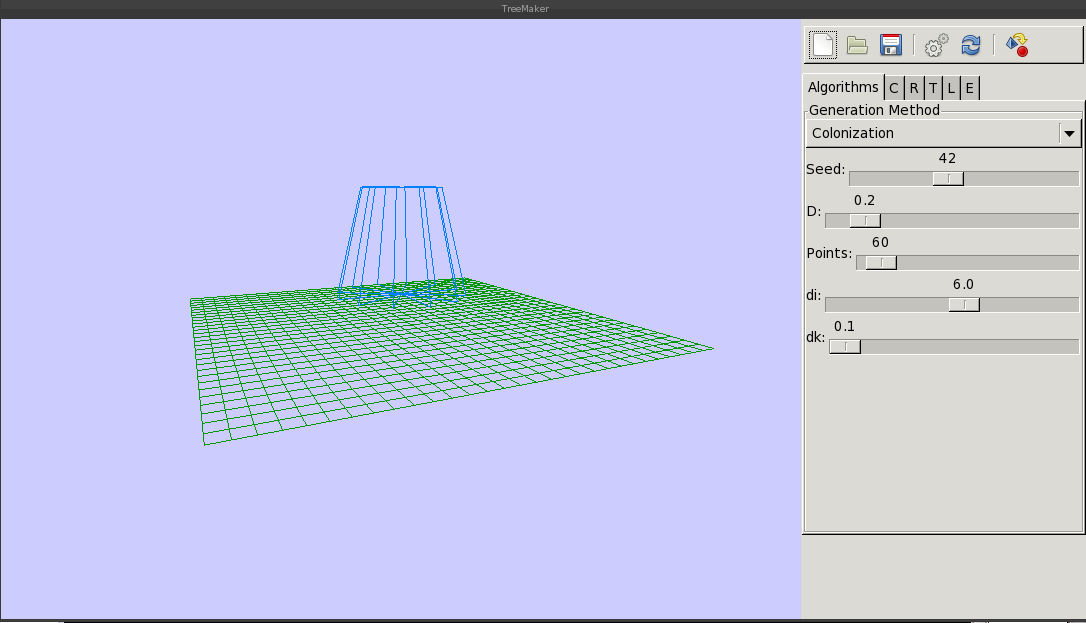
\includegraphics[width=140mm]{images/gui/mainWindow.png}}\\
\vspace{5mm}
Trzeba znalesc cos co ladnie zaznacza i maluje po takim obrazku zeby zaznaczyc widok drzewa dodac literke A i nadole opisac ze A to jest widok drzewa
Opis okna glownego: widok drzewa, panel opcji, toolbar
Opis toolbara, zapisu/odczytu/eksportu

A dalej to juz poszczególne zakładki z opisem, w sumie ze 3 strony
\subsection{Opcje korony}
\subsection{Opcje wyświetlania}
\subsection{Opcje pnia}
\subsection{Opcje liści}
\subsection{Edytor}
\section{Repozytorium git, buildowanie projektu, potrebne biblioteki}
